\documentclass{article}
\usepackage[utf8]{inputenc}
\usepackage[T1]{fontenc}
\usepackage[francais]{babel}
\usepackage{soul}
\usepackage{ulem}
\usepackage{amsmath}
\usepackage{amsmath}
\usepackage{amssymb}
\usepackage{mathrsfs}
\usepackage{amsthm}
\usepackage{pgfplots}

\usepackage{listings}
\lstset{
    language=R,
    basicstyle=\ttfamily
}
\setlength\parindent{0pt}


\pgfplotsset{compat=1.14}
\newcommand{\norm}[1]{\left\lVert#1\right\rVert^{2}}

\begin{document}

%--------------------------------------------------------------------------------
% PAGE DE GARDE
%--------------------------------------------------------------------------------

\begin{titlepage}

\newcommand{\HRule}{\rule{\linewidth}{0.5mm}} % lignes horizontales
\setlength{\topmargin}{0in}
\center % Center everything on the page
 
%----------------------------------
% Logos
\begin{minipage}{0.4\textwidth}
\begin{flushleft} \large
\hspace*{-0.5cm}
\end{flushleft}
\end{minipage}
~
\begin{minipage}{0.5\textwidth}
\begin{flushright} \large
\hspace*{1.5cm}
\end{flushright}
\end{minipage}\\[1cm]


%-----------------------------------
% Section d'entête
\textsc{\Large École Nationale de la Statistique et de l'Administration Économique}\\[1.5cm] 
\textsc{{\LARGE Rapport du Projet de Statistique}\\~\\Janvier 2017}\\[1cm]

%-----------------------------------
% Section de titre
\HRule \\[1cm]
{ \huge \bfseries Introduction à la régression pénalisée et à l'estimateur lasso}\\[0.4cm] % Titre
\HRule \\[1cm]
 
%------------------------------------
% Section des auteurs
\begin{minipage}{0.5\textwidth}
\begin{flushleft} \large
\emph{Auteurs:}\\
Mehdi \textsc{Abbana Bennani} \\
Julien \textsc{Mattei} \\
\end{flushleft}
\end{minipage}
~
\begin{minipage}{0.4\textwidth}
\begin{flushright} \large
\emph{Superviseur:} \\
Edwin \textsc{Grappin} \\[0.5cm] 
\end{flushright}
\end{minipage}\\[1.2cm]

%-------------------------------------
% Section de date
{\large \today}\\[0.5cm] % Date, change the \today to a set date if you want to be precise

\vfill % Fill the rest of the page with whitespace
\end{titlepage}

%---------------------------------------------------------------------------------
%  FIN PAGE DE GARDE
%---------------------------------------------------------------------------------

\title{	}

\section{Régression OLS}

\paragraph{Question 1 :}

\begin{align}
&\underset{\beta}{min}\norm{ y - X \beta} \tag{On minimise l'erreur quadratique}
\\ &\nabla_{\beta} \norm{ y - X \beta}(\beta^{\star}) = 0 \tag{Le gradient est nul en $\beta^\star$}
\notag \\ &\nabla_{\beta} ( y - X \beta)^{T} ( y - X \beta) (\beta^{\star}) = 0
\notag \\ &\boxed{\beta^{\star} = (X^{T}X)^{-1}X^{T}y}
\end{align}


Dans la suite on notera $\beta^{\star}$ l'estimateur des moindres carrés.

\paragraph{Question 2:}
~\par

Le code est disponible en annexe, pour cette question, nous avons divisé le dataset en un Train Set et en Test Set. La proportion du Train Set est de 90.\%
Ceci va nous permettre de mesurer l'erreur de prédiction.

La métrique que nous avons choisie pour mesurer cette erreur est la RMSE (Root Mean Square Error), définie par :
\begin{equation}
RMSE(\textbf{y}_{\textbf{test}}, \hat{\textbf{y}})= \frac{1}{|Test Set|}\sum_{i=1}^{|Test Set|}{(\hat{y}_{i} - y_{i})^2}
\end{equation}

Nous avons obtenu une RMSE de ... sur le test set avec l'estimation par moindre carrées. On remarque aussi qu'il n'y a aucun coefficient nul dans le paramètre $\star{beta}$ estimé.

Estimer la variance de l'erreur?

\paragraph{Question 3:}
~\par

On ne peut pas utiliser la régression par moindres carrés si le 
nombre de variables est supérieur au nombre d'observations
\begin{proof}
~\\Soit X est une matrice de dimensions (n,p)
\vspace{2mm} %5mm vertical space
\\On remarque que $X^{T}X$ est une matrice carrée de dimension p
\vspace{2mm} %5mm vertical space
\\ Par théorème : $rg(X) \leq min(n,p)$
\vspace{2mm} %5mm vertical space
\\Or $rg(X^{T}X) = rg(X)$
\vspace{2mm} %5mm vertical space
\\Donc $rg(X^{T}X) \leq min(n,p)$
\vspace{2mm} %5mm vertical space
\\Par hypothèse, le nombre de variables est plus grand que le nombre d'observations, soit $p > n$
\vspace{2mm} %5mm vertical spac
\\On a $rg(X^{T}X) < n $ car $min(n,p) = n$
\vspace{2mm} %5mm vertical spac
\\Donc $rg(X^{T}X) < p $ car $n < p$
\vspace{2mm} %5mm vertical spac
\\Ainsi $X^{T}X$ est une matrice de taille p dont le rang est strictement inférieur à sa dimension .
\vspace{2mm} %5mm vertical spac
\\Donc $X^{T}X$ n'est pas inversible.
\vspace{2mm} %5mm vertical spac
\\Conclusion : on ne peut pas utiliser la méthode des moindres carrées dans ce cas.
\end{proof}

\section{Régression pénalisée : le lasso}

\paragraph{Question 4 :}
~\par
\begin{align}
\intertext{Sous l'hypothèse de p=1, on résoud le problème d'optimisation:}
&\underset{\beta}{min}\frac{1}{2n} \|\textbf{y} - \textbf{X}\beta \|_{2} + \lambda\|\beta\|_{1} \notag
\intertext{En remplacant développant la norme 2 on obtient:}
&\underset{\beta}{min}\frac{1}{2n}\sum_{i=0}^{n}(y_{i}-x_{i}\beta)^2 + \lambda|\beta| \notag
\intertext{A partir de l'expression (1), on retrouve la valeur de l'estimateur par moindres carrés $\hat{\beta} = \frac{y}{x}$}
\intertext{On injecte $\hat{\beta}$ dans le problème d'optimisation:}
& \underset{\beta}{min} \frac{1}{2n}\sum_{i=0}^{n}x_{i}^{2}\beta^{2} - \frac{1}{n}\sum_{i=0}^{n}x_{i}^{2} \beta \hat{\beta} + \frac{1}{2n}\sum_{i=0}^{n}y_{i}^{2} +
\lambda|\beta| \notag
\intertext{On supprime les contantes:}
& \underset{\beta}{min} \frac{1}{2n}\sum_{i=0}^{n}x_{i}^{2}\beta^{2} - \frac{1}{n}\sum_{i=0}^{n}x_{i}^{2} \beta \hat{\beta} + \lambda|\beta| \notag
\intertext{On remarque que si $\hat{\beta}<0$ Alors forcément $\beta^{lasso}<0$
	Car les termes en $\beta^2$ et en $|\beta|$ ne dépendent pas du signe de $\beta$, et vu que $\hat{\beta}<0$ alors$\frac{1}{n}\sum_{i=0}^{n}x_{i}^{2} \hat{\beta}>0$ Donc pour minimiser la quantité, il faut que $\beta^{lasso}<0$  }
\intertext{De même si $\hat{\beta}>0$ Alors forcément $\beta^{lasso}>0$}
\intertext{On va traîter les deux cas:}
\intertext{Si $\hat{\beta}>0$, on résoud:}
& \underset{\beta}{min} \frac{1}{2n}\sum_{i=0}^{n}x_{i}^{2}\beta^{2} - \frac{1}{2n}\sum_{i=0}^{n}x_{i}^{2} \beta \hat{\beta} + \lambda\beta \notag
\intertext{On obtient $\beta^{lasso} = \hat{\beta} - \frac{\lambda}{\sum_{i=0}^{n}\frac{x_{i}^{2}}{2n}}$}
\intertext{Or $\beta^{lasso} $ forcément positif, donc $\beta^{lasso} = max(0, \hat{\beta} - \frac{\lambda}{\frac{1}{2n}\sum_{i=0}^{n}x_{i}^{2}})$}
\intertext{Si $\hat{\beta}<0$, à l'aide d'un raisonnement similaire $\beta^{lasso} = max(0, \hat{\beta} + \frac{\lambda}{\frac{1}{2n}\sum_{i=0}^{n}x_{i}^{2}})$}
\intertext{On en déduit que $\beta^{lasso} = sg(\hat{\beta}) (|\hat{\beta}| - t )_{+}$ avec $t = \frac{\lambda}{\frac{1}{2n}\sum_{i=0}^{n}x_{i}^{2}}$}
\end{align}

Le seuillage doux permet de regler l'intervalle sur lequel on veut estimer $\beta^{\star}$. Ainsi, on choisit $\lambda$, si notre estimateur $\beta^{\star}$ est compris dans l'intervalle $[-\lambda,\lambda]$ il est ramené à 0. On ne retient que les valeurs de $\beta^{\star}$ en dehors de cet intervalle (même principe qu'un filtre).
\\L'estimateur $\hat{\beta}^{lasso}$ est nul pour tout les $\beta^{\star}$ tels que $\beta^{\star} - t < 0$. Donc cela induit une estimation nulle plus souvent que l'estimateur des moindres carrés (qui se produit seulement lorsque $\beta^{\star} = 0$)

\begin{tikzpicture}
\begin{axis}[ 
xlabel=$\hat{\beta}$,
ylabel={$sg(\hat{\beta}) (|\hat{\beta}| - 2 )_{+}$}
] 
\addplot {x/ abs(x) *(max(abs(x) - 2, 0))}; 
\end{axis}
\end{tikzpicture}

\paragraph{Question 5:}
~\par
Dans la régression pénalisée, on pénalise les valeurs de $\beta$ pour limiter leur valeurs possibles, dans le cas du lasso par exemple, toutes les estimations par moindres carrées inférieures à t sont ramenées  zeros, l'intervalle d'estimation est $\left\lbrace0\right\rbrace\cup$$[t,\infty[$. Dans le cas de la régression Ridge par exemple, on pénalise les coefficients trop grands.
\\ L'estimateur Lasso est adapté à notre problème car nous allons pouvoir réduire la taille de l'espace des paramètres jusqu'à ce que le nombre de coefficients de beta non nuls soit égal à n (le nombre d'observations), en changeant la valeur de $\lambda$. Plus celui-ci est grand, plus le nombre de paramètres nuls sera grand.



\paragraph{Question 6 :}
~\par

Quelles sont les avantages du lasso sur la pénalisation ` 0 ?
Même question avec la pénalisation Ridge

La pénalisation Ridge a tendance à pénaliser les valeurs dans $\beta$ trop grandes, mais n'a pas tendance à maximiser le nombre de paramètres nuls, contrairement à la pénalisation l0.

\paragraph{Question 7 :}
~\par
Faire un commentaire

\paragraph{Question 8 :}
~\par

Le parametre $lambda$ permet de régler le nombre de coefficients nuls dans $\beta^{lasso}$.

\paragraph{Question 9 :}
~\par

Dans la méthode de cross validation, on divise le dataset en trois parties: 
Train Set, Validation Set, et Test Set.
On entraine le modèle sur le train set puis on estime la qualité de la prédiction sur le validation set pour plusieurs valeurs de $\lambda$, on choisit le lambda le plus performant sur le validation set. Esuite on estime le modèle avec cette valeur de $\lambda$ sur le train set comprenant le train set précédent et le validation set précédent.

\paragraph{Question 10 :}
~\par

Pour évalueer l'erreur du modèle, nous avons divisé la base de données en Train Set et Test Set, les données du Train Set sont utilisées pour estimer les paramètres, les données du test set sont ensuite utilisés pour évaluer l'erreur d'estimation. La mesure que nous utiliserons est la Root Mean Square Error, RMSE, définie par :
\begin{equation}
RMSE(\textbf{y}_{\textbf{test}}, \hat{\textbf{y}})= \frac{1}{|Test Set|}\sum_{i=1}^{|Test Set|}{(\hat{y}_{i} - y_{i})^2}
\end{equation}

\begin{figure}[ht]
   \caption{\label{nb_zeros_cval} Nombre de zéros dans $\beta^{lasso}$ en fonction de $\lambda$, avec $\beta^{lasso} de taile 400$}
   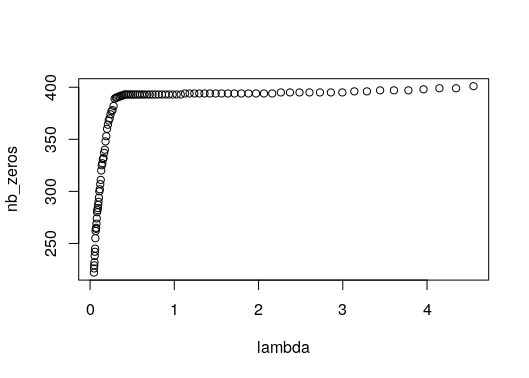
\includegraphics[scale=0.5]{nb_zeros_cval.png}
\end{figure}



\newpage
\section{Appendix}

\lstinputlisting[numbers=left, breaklines=true]{main.R}


\end{document}